\begin{usecase}{06}{Gestione del dettaglio tecnico sul regolatore semaforico}
\usecaseprimaryactors{Utente autenticato}
\usecasepre{L'utente sta visionando il dettaglio del regolatore semaforico selezionato dalla lista.}
\usecasedesc{L'utente può gestire il dettaglio tecnico del regolatore semaforico, visualizzandolo e aggiungendo note.}
\usecasepost{L'utente può gestire il dettaglio tecnico del regolatore semaforico, visualizzandolo e aggiungendo note.}
\label{uc:UC06}
\end{usecase}

\begin{figure}[!h] 
    \centering 
    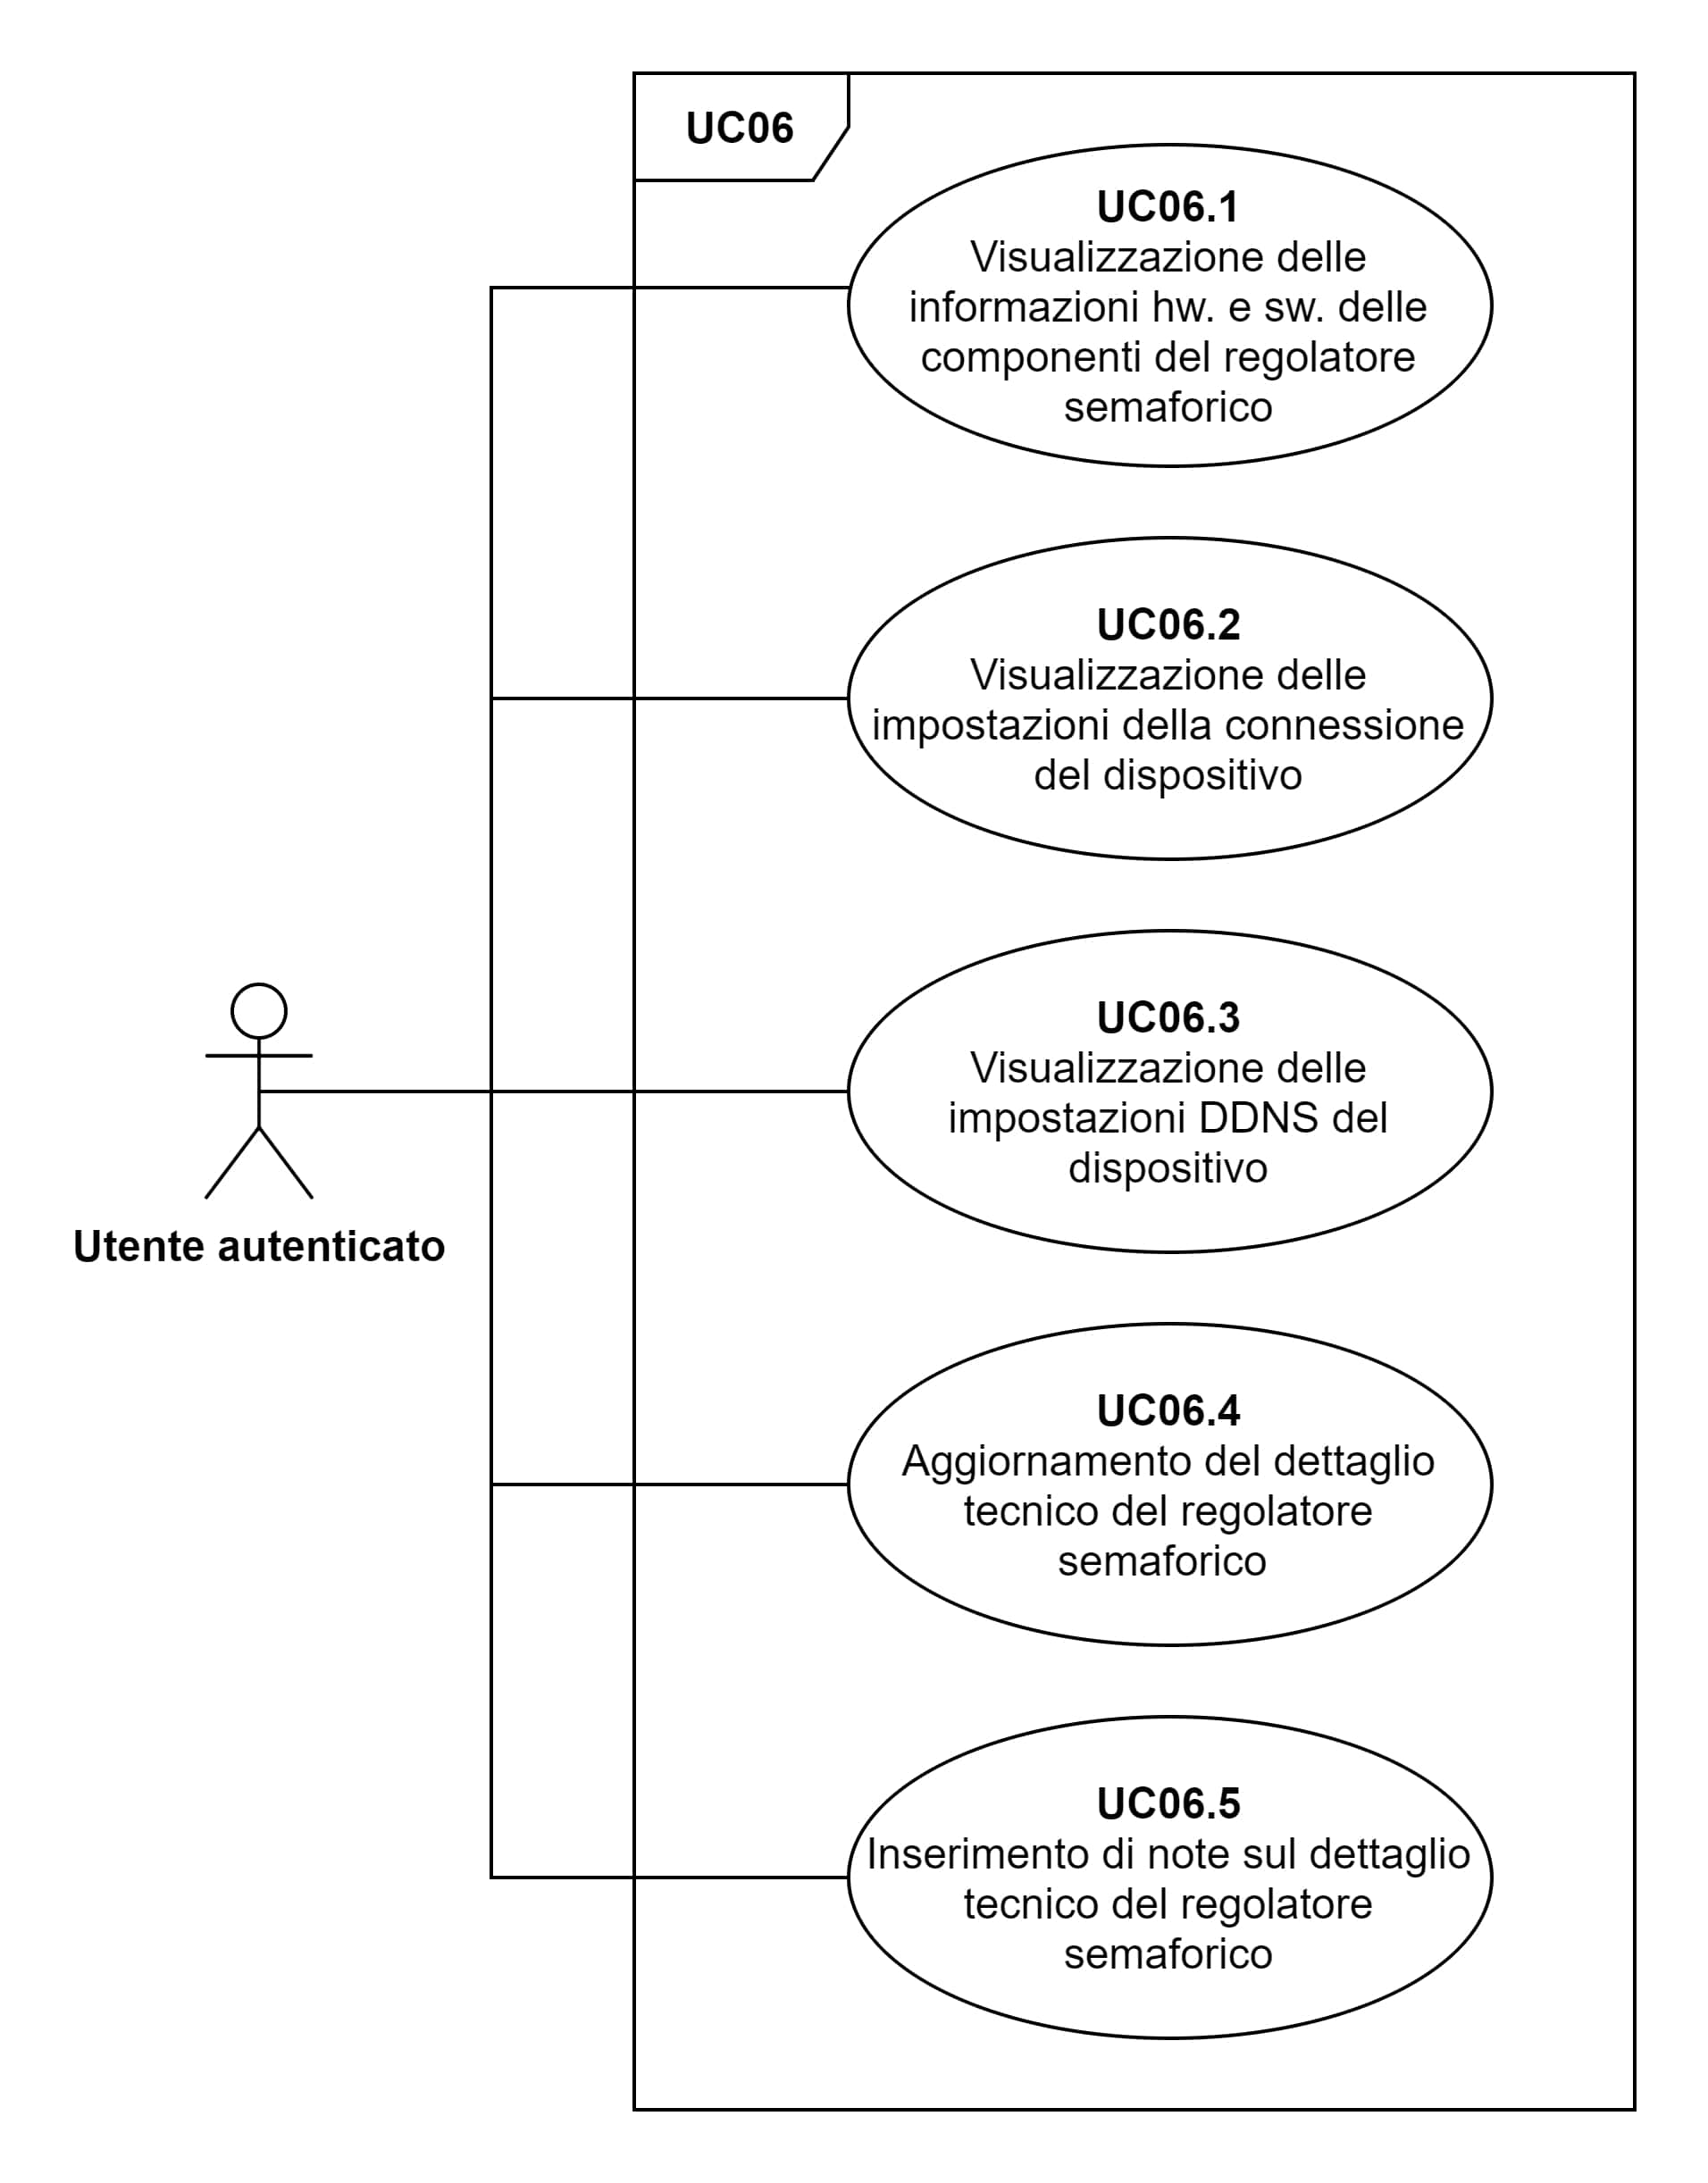
\includegraphics[width=1.0\columnwidth]{appendice-A/uc06} 
    \caption{SMacs - Sotto-casi d'uso di UC06 - Gestione del dettaglio tecnico sul regolatore semaforico}
\end{figure}

\begin{usecase}{06.1}{Visualizzazione delle informazioni hardware e software delle componenti del regolatore semaforico}
\usecaseprimaryactors{Utente autenticato}
\usecasepre{L'utente sta visionando il dettaglio tecnico del regolatore semaforico.}
\usecasedesc{Vengono visualizzate le informazioni hardware e software delle componenti del regolatore semaforico.}
\usecasepost{Vengono visualizzate le informazioni hardware e software delle componenti del regolatore semaforico.}
\label{uc:UC06-1}
\end{usecase}

\begin{usecase}{06.2}{Visualizzazione delle impostazioni della connessione del dispositivo}
\usecaseprimaryactors{Utente autenticato}
\usecasepre{L'utente sta visionando il dettaglio tecnico del regolatore semaforico.}
\usecasedesc{Vengono visualizzati l'indirizzo IP e la porta a cui il dispositivo è raggiungibile.}
\usecasepost{Vengono visualizzati l'indirizzo IP e la porta a cui il dispositivo è raggiungibile.}
\label{uc:UC06-2}
\end{usecase}

\begin{usecase}{06.3}{Visualizzazione delle impostazioni DDNS del dispositivo}
\usecaseprimaryactors{Utente autenticato}
\usecasepre{L'utente sta visionando il dettaglio tecnico del regolatore semaforico.}
\usecasedesc{Vengono visualizzate le impostazioni DDNS del dispositivo.}
\usecasepost{Vengono visualizzate le impostazioni DDNS del dispositivo.}
\label{uc:UC06-3}
\end{usecase}

\begin{usecase}{06.4}{Aggiornamento del dettaglio tecnico del regolatore semaforico}
\usecaseprimaryactors{Utente autenticato}
\usecasepre{L'utente sta visionando il dettaglio tecnico del regolatore semaforico.}
\usecasedesc{L'utente seleziona la funzionalità di aggiornamento e viene aggiornato il dettaglio tecnico del regolatore semaforico.}
\usecasepost{L'utente seleziona la funzionalità di aggiornamento e viene aggiornato il dettaglio tecnico del regolatore semaforico.}
\label{uc:UC06-4}
\end{usecase}

\begin{usecase}{06.5}{Inserimento di note sul dettaglio tecnico del regolatore semaforico}
\usecaseprimaryactors{Utente autenticato}
\usecasepre{L'utente sta visionando il dettaglio tecnico del regolatore semaforico.}
\usecasedesc{L'utente seleziona la funzionalità di inserimento di note sul dettaglio tecnico del regolatore semaforico e inserisce delle note.}
\usecasepost{L'utente seleziona la funzionalità di inserimento di note sul dettaglio tecnico del regolatore semaforico e inserisce delle note.}
\label{uc:UC06-5}
\end{usecase}